
\documentclass[11pt]{beamer}
\usepackage{helvet} %font
\beamertemplatenavigationsymbolsempty
\usetheme{JuanLesPins}
\usefonttheme{structurebold}

\usepackage[french]{babel}
\usepackage[utf8]{inputenc}
\usepackage[T1]{fontenc}
\usepackage{amssymb,amsmath}
\usepackage{tikz}
\usepackage{geometry}
\usepackage{xcolor,colortbl}
\usetikzlibrary{arrows,positioning}
\usepackage{listings}

\AtBeginSubsection[]
{
   \begin{frame}
	\small \tableofcontents[currentsection]
   \end{frame}
}

\newenvironment{slide}[1]{%
\begin{frame}[environment=slide]
\frametitle{#1}
}{%
\end{frame}
}
\setbeamercolor{structure}{fg=red}
\setbeamercolor{frametitle}{bg=black,fg=white}
\definecolor{gris}{gray}{0.6}
\definecolor{grisclair}{gray}{0.9}

\newtheorem{exercice}{Exercice}

\title{Machine Learning I \\ Introduction à \texttt{pandas}}
\author{Nicolas Bourgeois}
\date{}

\newcommand{\Python}[1]{
	{\small	\lstinputlisting[language=Python]{./#1.py}}
}
\newenvironment{pyenvsmall}
	{ \ttfamily \tiny }
	{\par  }

\newcommand{\Pythonsmall}[1]{
	{\scriptsize \lstinputlisting[language=Python]{./#1.py}}
}
\newcommand{\elimine}[1]{{\textcolor{lightgray}{#1}}}

\newcommand\Wider[2][3em]{%
\makebox[\linewidth][c]{%
  \begin{minipage}{\dimexpr\textwidth+#1\relax}
  \raggedright#2
  \end{minipage}%
  }%
}

\begin{document}




\begin{frame}{Exercice}
\begin{exercice}
Chargez le fichier \texttt{data1.csv} dans une table. Identifiez quelles sont les colonnes qui contiennent le plus de valeurs manquantes.
\end{exercice}

\begin{exercice}
Supprimez les colonnes avec valeurs manquantes et affichez les cinq premières lignes. Que se passe-t-il si vous éliminez les plutôt les lignes avec valeurs manquantes ?
\end{exercice}

\begin{exercice}
Affichez cinq lignes aléatoires (doublons autorisés).
\end{exercice}
\end{frame}


\begin{frame}{Exercice}
\begin{exercice}
Produisez la sous-table des passagers de 1ere classe.
\end{exercice}
\begin{exercice}
Produisez la sous-table des passagers masculins d'âge compris entre 30 et 50 inclus.
\end{exercice}
\begin{exercice}
A l'aide de \texttt{groupby}, trouvez l'effectif, l'âge moyen et le taux de survie des passagers par classe.
\end{exercice}
\end{frame}



\begin{frame}{Problème}
\begin{exercice}
Dans le fichier \texttt{data2.csv}, trouvez le total cumulé de développement des provinces contrôlées par Muscovy, Ryazan et Novgorod qui ne produisent pas de céréales ('Grain').
\end{exercice}
\begin{exercice}
Même question mais en appliquant préalablement une fonction qui diminue pour chaque province produisant de la fourrure ('Fur') le développement de 5, sans toutefois pouvoir le descendre en dessous de 3.
\end{exercice}
\end{frame}


\begin{frame}{Exercice}
\begin{exercice}
Importez sur un serveur la base de données data3.sql. Puis avec une interface de type MySQLdb, lisez-la avec pandas sous forme d'un dictionnaire de dataframes (la clef étant le nom).
\end{exercice}
\end{frame}


\begin{frame}{Exercice}
\begin{exercice}
Dans la table des personnages, ne gardez que les champs \texttt{'id'}, \texttt{'name'} et \texttt{'date\_start'}, puis éliminez les lignes avec valeurs manquantes.
\end{exercice}

\begin{exercice}
Faites trois joins de cette table avec les tables appropriées de façon à ajouter des colonnes mentionnant le titre complet de chaque personnage, par exemple :\\ 

\quad "Louis le Pieux, roi, Aquitaine".
\end{exercice}
\end{frame}

\begin{frame}{Exercice}
\begin{exercice}
Affichez les fonctions $x \mapsto e^{-\lambda x}$ pour diverses valeurs du paramètre $\lambda$. N'oubliez pas l'axe et la légende.
\end{exercice}

\begin{exercice}
Même question, mais les courbes doivent être sur des sous-figures différentes et non superposées.
\end{exercice}
\end{frame}

\begin{frame}{Résultat attendu (1)}
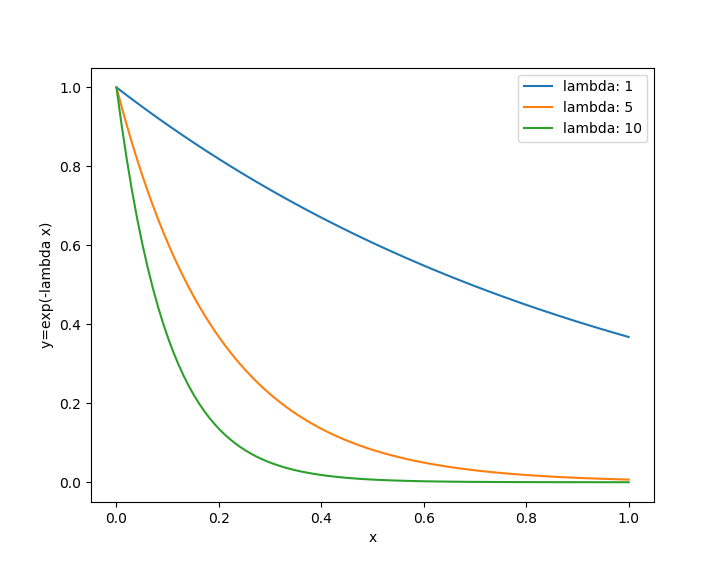
\includegraphics[scale=0.45]{ex201}
\end{frame}

\begin{frame}{Résultat attendu (2)}
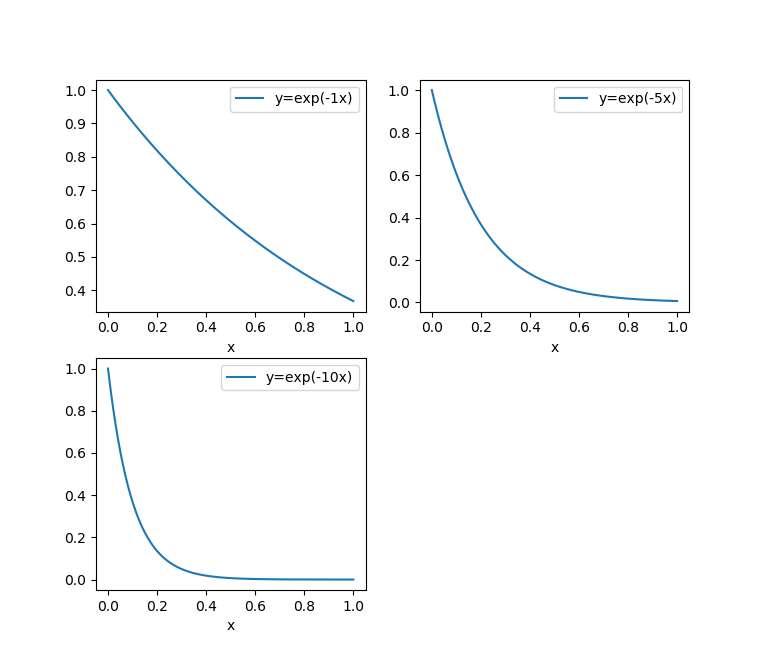
\includegraphics[scale=0.45]{ex202}
\end{frame}


\begin{frame}{Exercice}
\begin{exercice}
Reprenez les courbes du premier exercice et annotez-les pour distinguer les points $y=e^{-1}$.
\end{exercice}
\end{frame}

\begin{frame}{Résultat attendu}
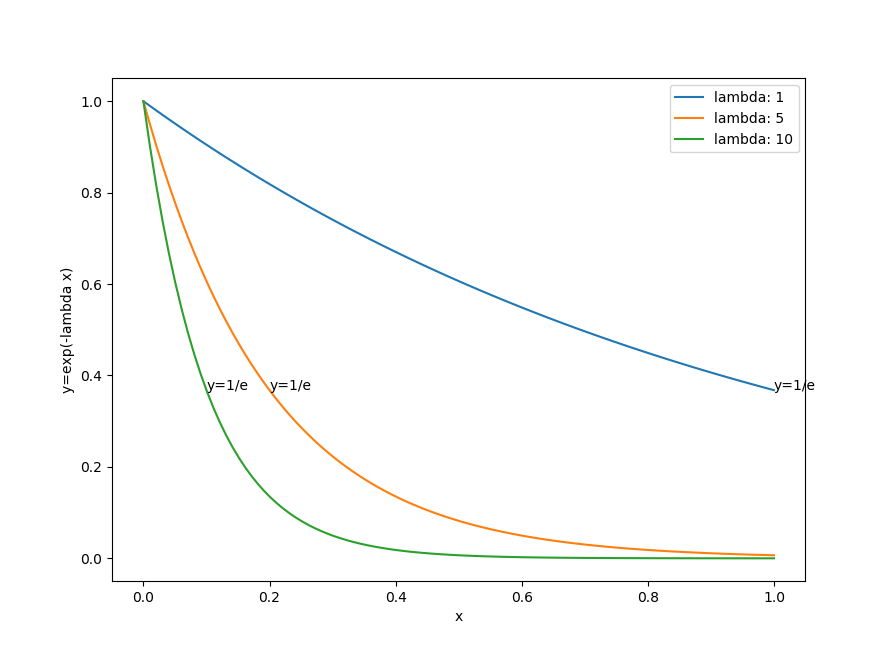
\includegraphics[scale=0.45]{ex203}
\end{frame}


\begin{frame}{Exercice}
\begin{exercice}
Importez les données de data1.csv dans un dataframe et affichez leur dispersion selon les axes age et prix du billet.
\end{exercice}
\begin{exercice}
Modifiez la couleur et ajoutez une légende de façon à faire apparaître l'information si la personne a survécu ou non.
\end{exercice}
\end{frame}

\begin{frame}{Résultat attendu (1)}
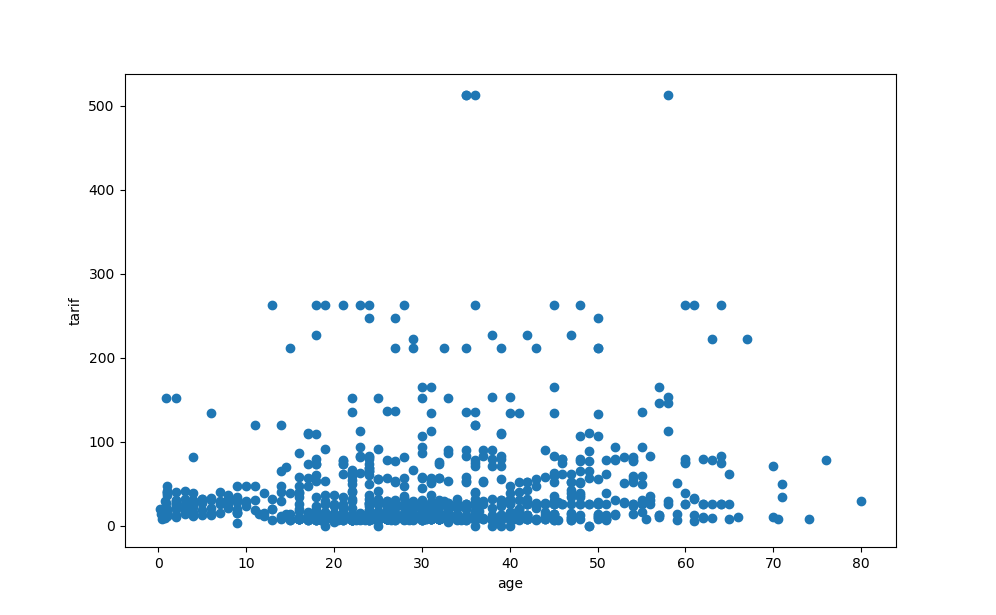
\includegraphics[scale=0.45]{ex203bis}
\end{frame}

\begin{frame}{Résultat attendu (2)}
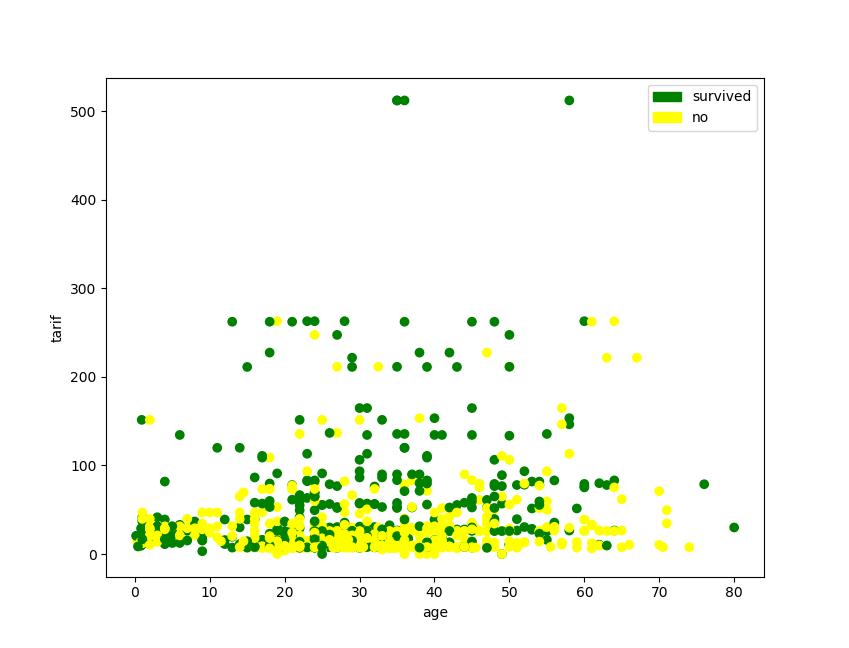
\includegraphics[scale=0.45]{ex204}
\end{frame}

\end{document}